% chapter Methods/Design

\section{Approach Adopted}

Grid performance monitoring in this project is examined using {\bf GMA}, an architecture introduced to provide the standards for a distributed monitoring system. The technologies that will be discussed here are about the Information Infrastructure that provides the metrics to the users/applications.

The metrics are generated using {\bf Linux kernel}'s load average functions. {\bf Ganglia} is used to take these metrics and synchronize all cluster nodes with the relevant information, over the {\bf multicast channel}.

Nagios is configured using a {\bf custom script} that takes the information for the cluster nodes, and periodically queries the {\bf Gmond} to get the metrics for the discovered nodes. The results are stored in its repository and using RRDTool and PNP4Nagios, graph reports are generated on demand.

To pass the information, two different information systems are examined, {\bf BDII and WSRF}. Both are used in modern grid implementations and are described in {\bf MDS specification}. BDII queries event source (Gmond) using Perl/Python LDAP libraries. The results taken, fill the directory schema which has been extended using {\bf Glue schema} specification for Processor Load in Computing Element structure.

{\bf MDS4} introduces the use of {\bf WSRF} in grid information system. A {\bf Ganglia Information Provider} using {\bf XSLT} takes the XML output from Gmond and aggregates the metrics using WSRF {\bf Aggregation Framework}. In front of it, a Tomcat instance serves the {\bf WebMDS} frontend to allow {\bf XPath} queries to the results that have been aggregated.

Finally, two sample small applications has been developed to provide a homogeneous interface that displays the same information using the two different information systems.

\begin{figure}[htb]
\centering
 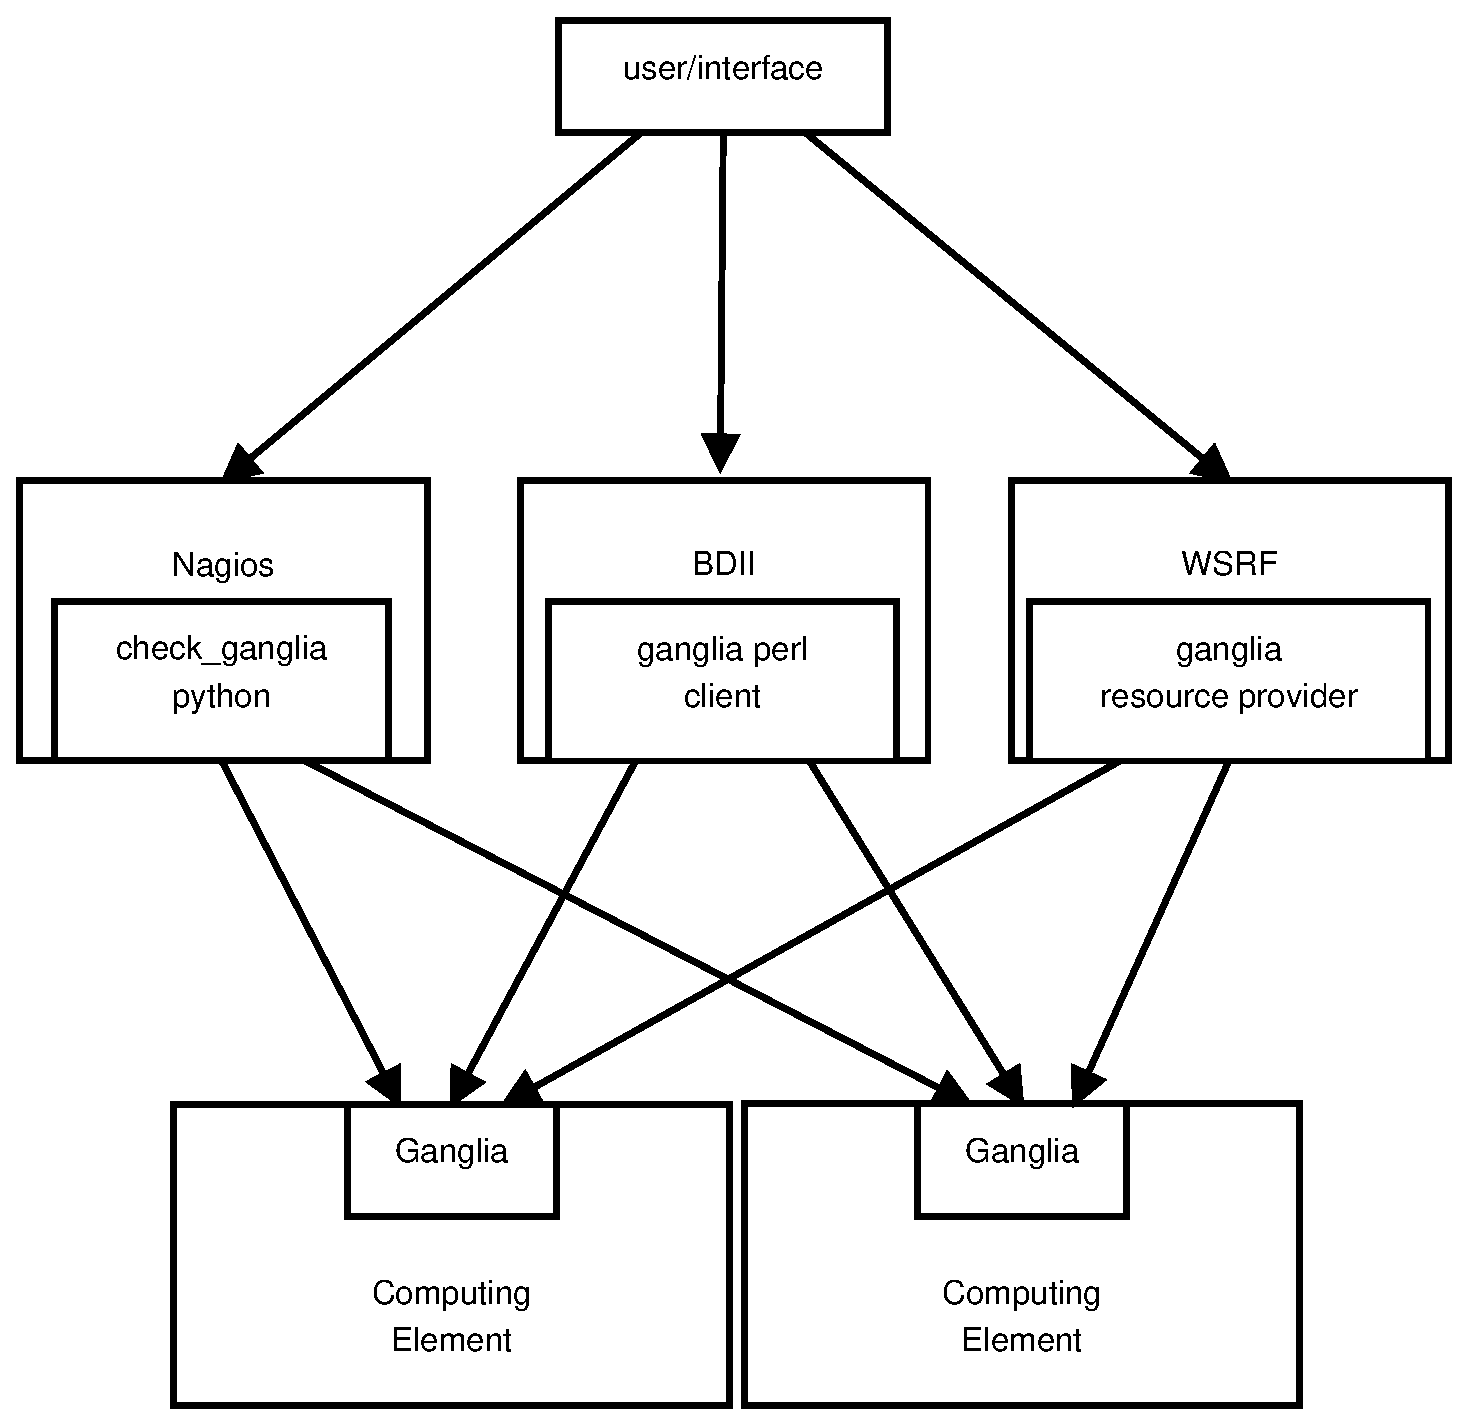
\includegraphics[width=130mm]{images/is.eps}
\caption{Overview of Information Systems used to monitor the grid}
\label{figure:is}
\end{figure}

\section{Design Methods}

\subsection{Grid Monitoring Architecture}

By definition \cite{Taylor2006} Grid Monitoring Architecture consists of three components, as shown in Figure \ref{figure:gma}:
\nomenclature{GMA}{Grid Monitoring Architecture}

\begin{enumerate}
\item {\bf Directory Service} which supports the publishing and discovery of the information
\item {\bf Producer component}: which is responsible for the availability of the performance data that takes from the event source and
\item {\bf Consumer component}: the one that requests the performance data and receives the metrics from the producer.
\end{enumerate}

\begin{figure}[htb]
\centering
 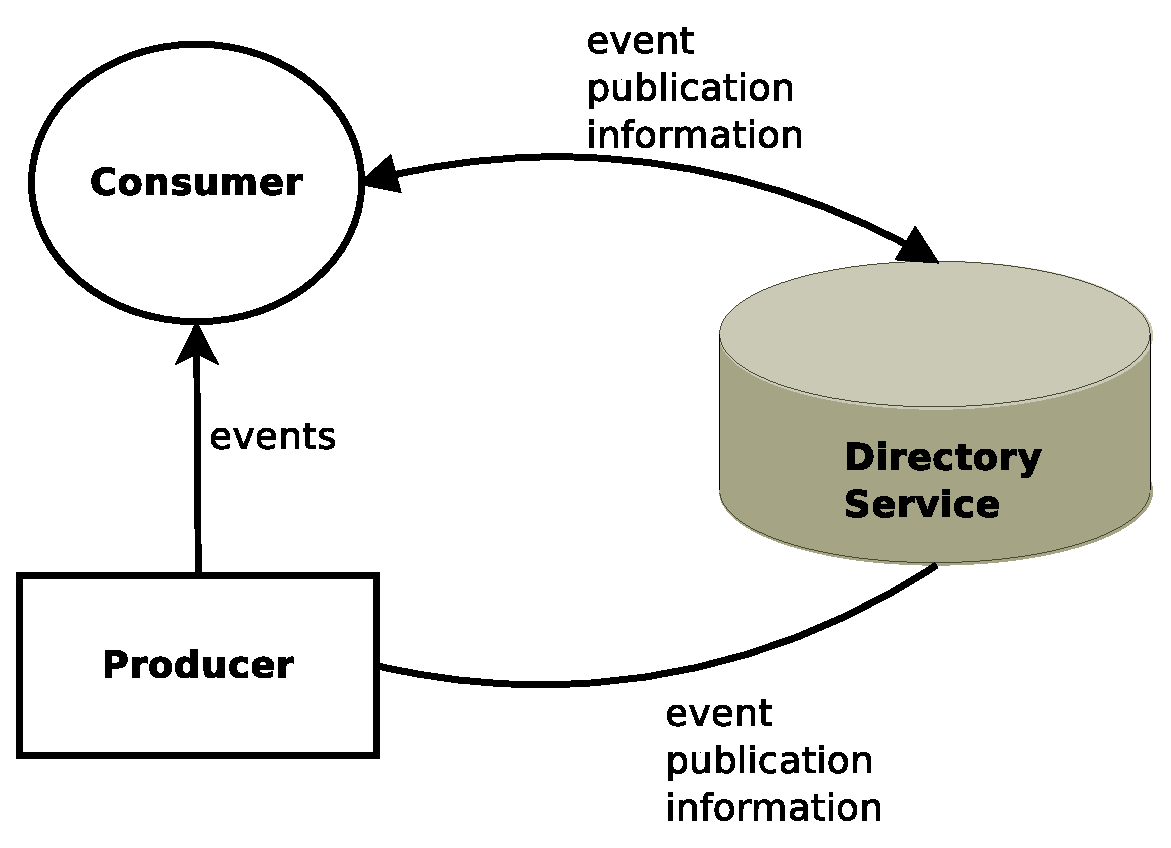
\includegraphics[width=100mm]{images/gma.eps}
\caption{Grid Monitoring Architecture}
\label{figure:gma}
\end{figure}

In GMA, all metrics that are transmitted by the producer are handled as events with a timestamp, so performance data should be accurate. These events are transmitted to the consumer directly, and not through the directory service (whose role is just to advertise producers to consumers and vice versa). The GMA recommends that the structure of these data should be following a schema definition. 

Grid Monitoring Architecture supports two models to handle the communication between producers and consumers:

\begin{itemize}
\item {\bf Streaming publish/subscribe model}
\item {\bf Query/Response model}
\end{itemize}

The directory service is used by producers to discover consumers and by consumers to discover producers. The information of the availability of each producer/consumer is published to the directory service. Each component may initiate a connection to another type of component which has been discovered in the directory service. Even though the role of the directory service is centralized in the discovery of components between each other, the performance data messages are transferred between the producer/consumer directly and not via the Directory Service.

\subsection{GLUE Schema}

GLUE schema came to provide the interoperability needed between US and European Physics Grid Projects. As a standard, a common schema was introduced to describe and monitor the grid resources. Major components include:

\begin{itemize}
\item Computing Element (CE)
\item Storage Element (SE)
\item Network Element (NE)
\end{itemize}

The implementation of Glue schema may be using LDAP, XML or SQL. The MDS implementation of the Glue schema in this project includes the core Information Provider and the Ganglia Interface for the cluster information.

\nomenclature{GLUE}{Grid Laboratory Uniform Environment}

\begin{figure}[htb]
\centering
 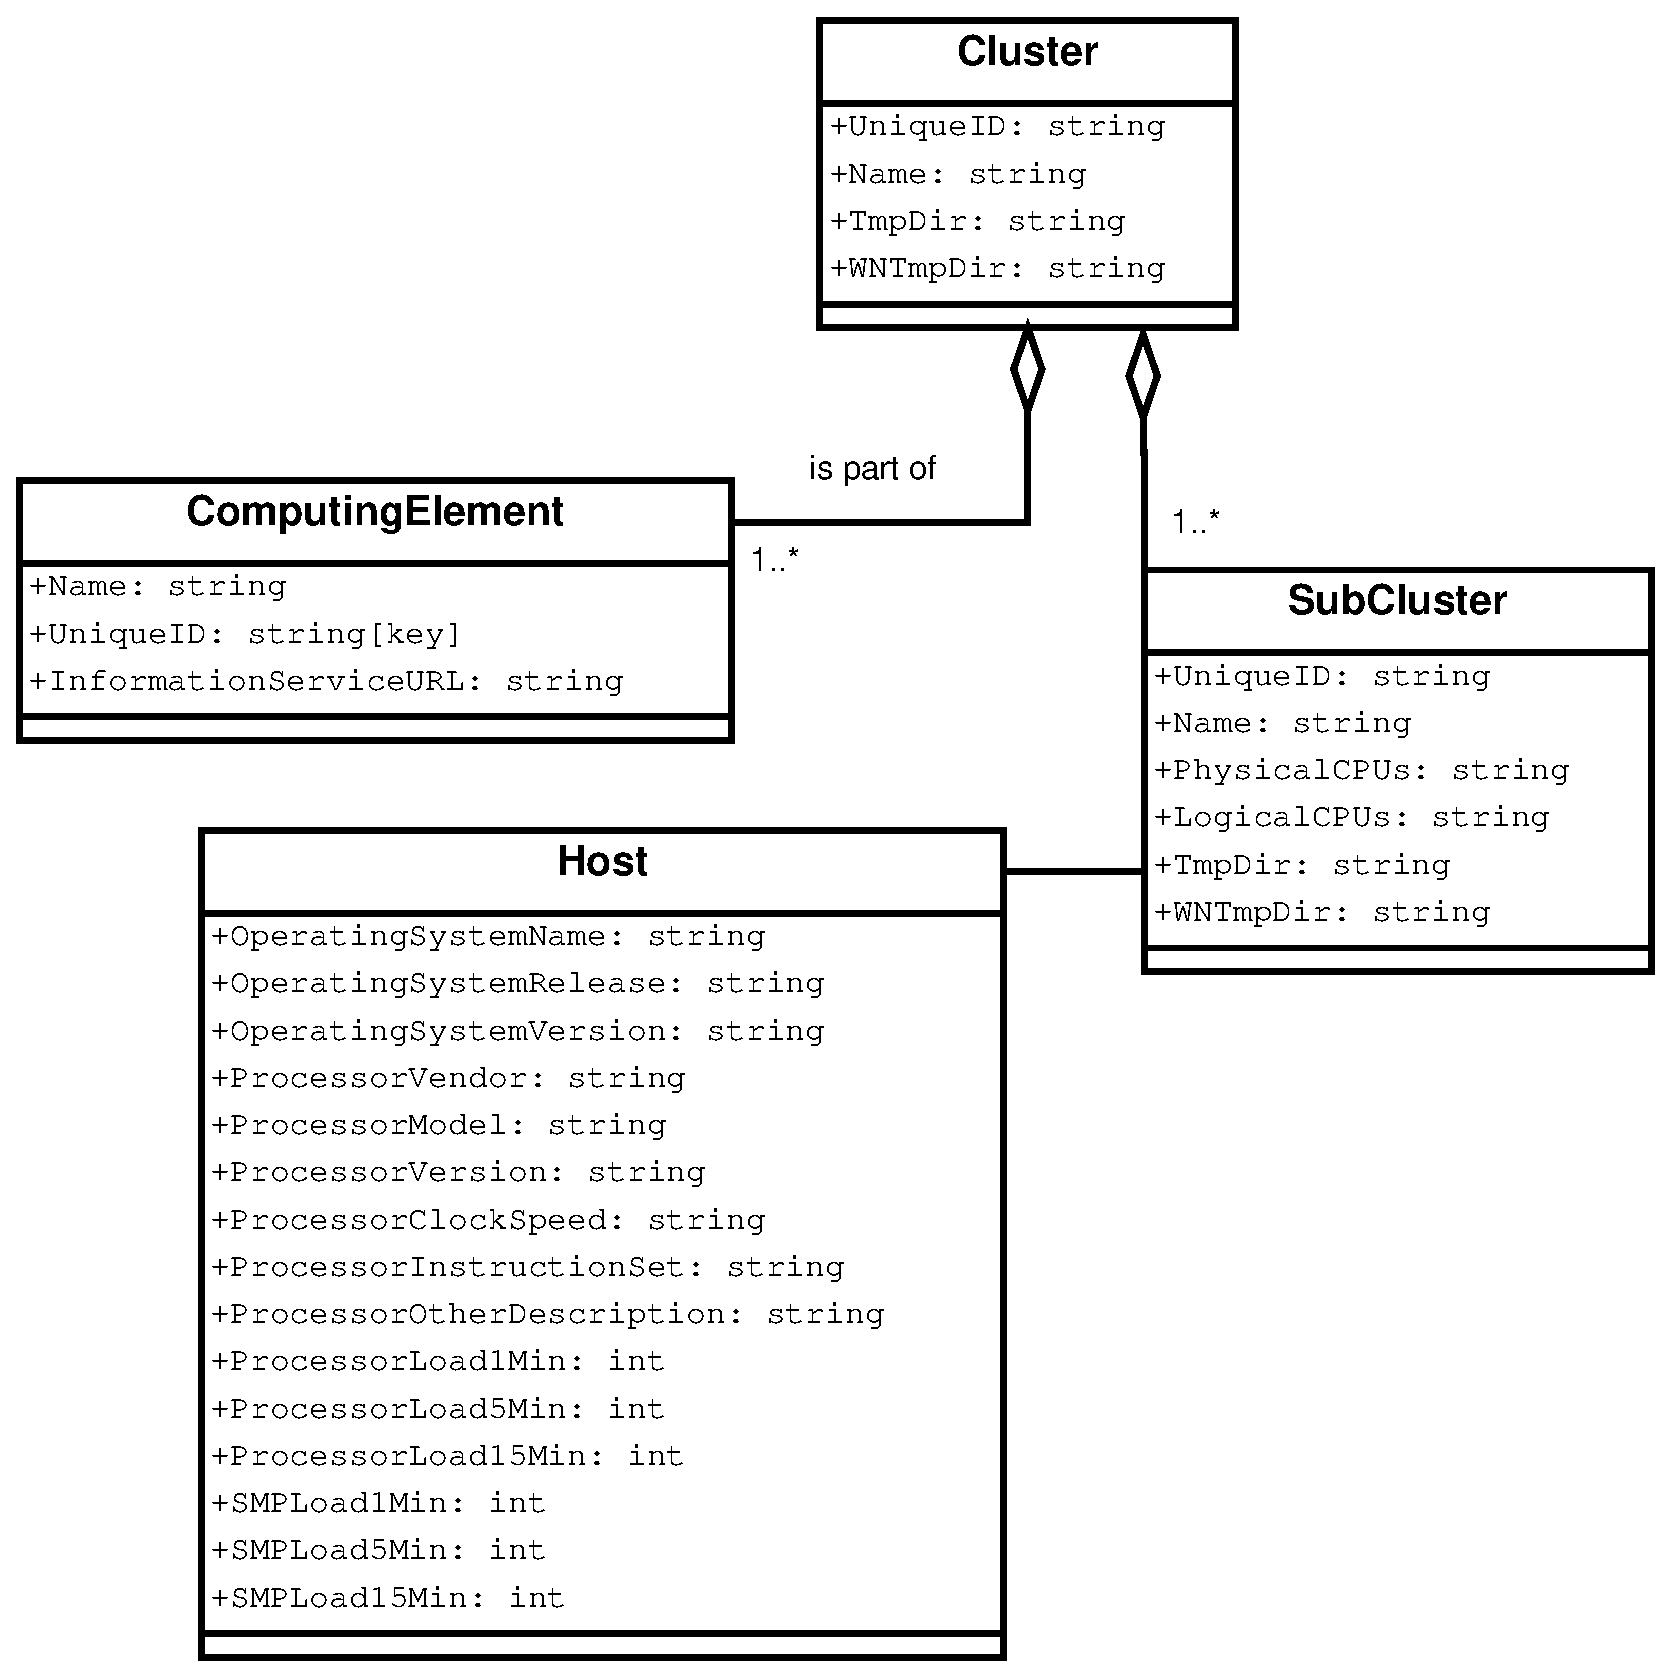
\includegraphics[width=130mm]{images/gluece_ext.eps}
\caption{GLUE schema 2.0 extension for Host and SMP Load}
\label{figure:gluece_ext}
\end{figure}


\subsection{Information Infrastructure}

Because grid computing applications usually operate in large scale installations, there are performance requirements for the information infrastructure, such as performance, scalability, cost and uniformity. Rapid access to configuration information that is frequently used, should be enhanced using {\bf caching to query periodically each host or index server for the metrics}.

The number of components in a grid infrastructure scales up to hundreds of thousands of nodes, and these components should be available for queries by many different tools. That information should be discoverable using information indexes.

Deployments, maintenance and operations in a large installation of many systems have operational costs for human resources. The information system should automatically discover and serve the availability paths for applications and grid resources/services.

Because of the large number of different heterogeneous networks of nodes and clusters, there is a need of uniformity. Uniformity helps developers to build applications that give better configuration decisions, by simplification, to build APIs for common operations and data models for the representation of that information. Resources are divided in groups of computing, storage, network elements, etc.

The solution proposed by GLUE standard and X.500 (Directory Service) is the key feature to scale, and get uniformity. It may be used to provide extensible distributed directory services. It is optimized for reads, its binary-tree like hierarchy and usually back-end data structure provides a framework that well organizes the information that need to be delivered by an Information Infrastructure.\cite{mds1}

\section{Data-acquisition Systems}

\subsection{Metrics}\label{subsec:metrics}

{\bf CPU load} is taken using the pseudo /proc/loadavg file which in turn is
filled by Linux kernel's CALC\_LOAD macro. This function takes 3 parameters:
The load-average bucket, a $y$ constant that is calculated using formula
\[
y=\frac{2^{11}}{2^{((5log_2(e))/60x)}}
\]
for values $x=1$, $x=5$ and $x=15$ (where x represent the minutes and y the
exponent constant), and the number of how many processes are in the queue, in
running or uninterruptible state.

\begin{figure}[htb]
\centering
 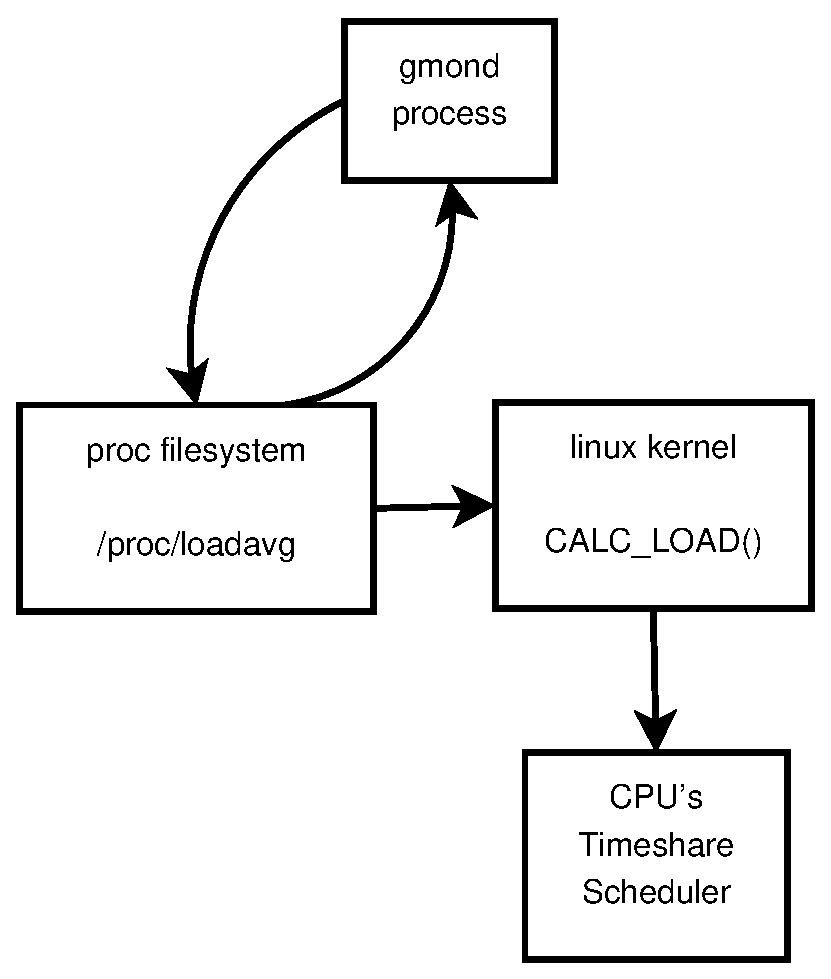
\includegraphics[width=80mm]{images/calc_load.eps}
\caption{Load Average calculation}
\label{figure:calc_load}
\end{figure}


\subsection{Ganglia}\label{subsec:ganglia}

The metrics about load in one, five and fifteen minutes are taken from Gmond daemon through the proc filesystem as seen in Figure \ref{figure:calc_load}. These values are multicasted using a UDP message on the network, only if the value has been changed from the previous one taken. There is also a time threshold that after that time the value is been sent again, even if it haven't changed, so new hosts on the network may gather the data needed for their Gmond. Each host of a cluster have the information about the metrics of itself and each other node, so it stores the whole cluster state. Using loopback interface, every Gmond sends its metrics to itself.

If a TCP connection on the Gmond listening port 8649 is made, Gmond writes a full cluster state of metrics in XML including its DTD. There is a typical access list in the configuration called trusted hosts, where every node of that cluster is allowed to connect to get the XML.

\begin{figure}[htb]
\centering
 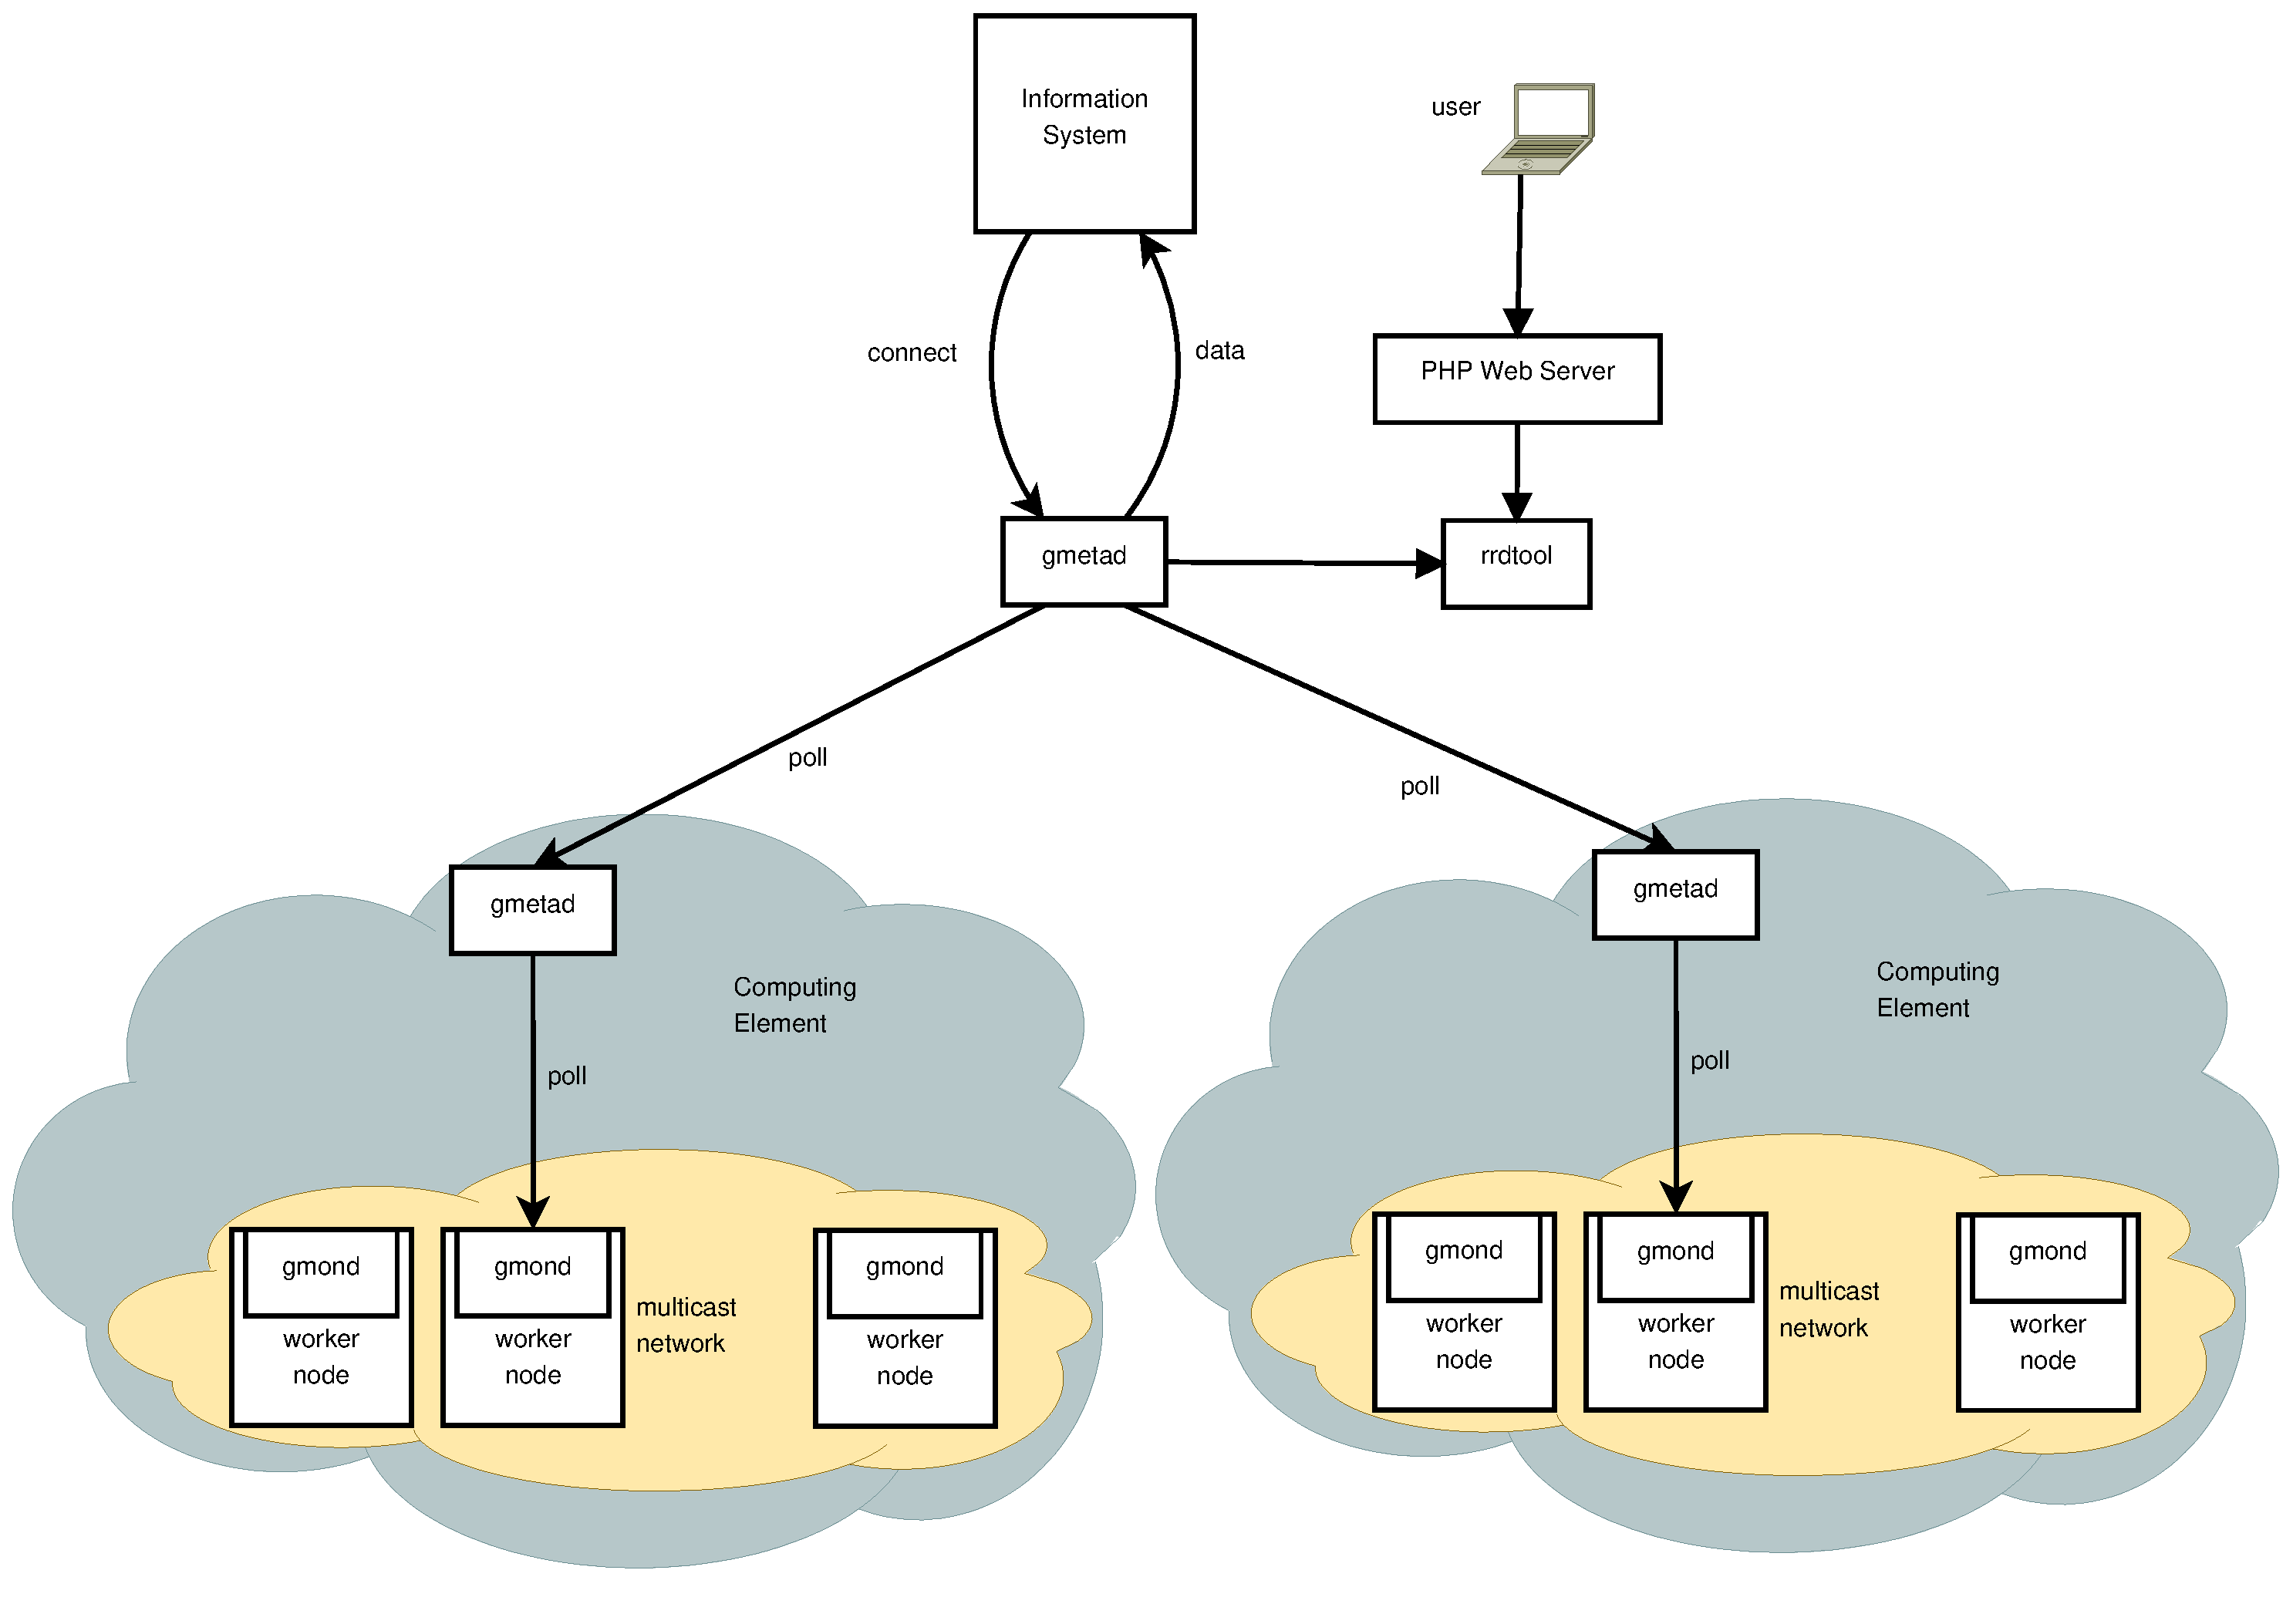
\includegraphics[width=130mm]{images/ganglia_data_flow.eps}
\caption{Ganglia Network Communications}
\label{figure:ganglia_network}
\end{figure}

\subsubsection{Installation and configuration}

In order to install ganglia, some dependencies were needed to be installed on each node of the Computing Element. In the testbed, there were an installation of LTSP \cite{ltsp} and the quick deployment of ganglia succeeded. Ganglia sources compiled for Gmond on the nodes and Gmetad on the systems that Ganglia Web interface needed to be installed. Finally on worker nodes, iptables should accept connections on 8649/TCP port.

\begin{lstlisting}
# yum install rrdtool perl-rrdtool rrdtool-devel apr-devel libconfuse libconfuse-devel expat expat-devel pcre pcre-devel
# GANGLIA_ACK_SYSCONFDIR=1 ./configure --with-gmetad
# make
# make install
# mkdir -p /var/lib/ganglia/rrds
# chown -R nobody /var/lib/ganglia
\end{lstlisting}

\begin{lstlisting}
# yum install apr-devel libconfuse libconfuse-devel expat expat-devel pcre pcre-devel
# GANGLIA_ACK_SYSCONFDIR=1 ./configure
# make
# make install
# iptables -A RH-Firewall-1-INPUT -m state --state NEW -m tcp -p tcp --dport 8649 -j ACCEPT
\end{lstlisting}

Gmond and Gmetad default configuration may be generated using the daemon itself. Gmond may be configured using multicast to communicate metrics between nodes or unicast to solve problems with jitter when deployed in environments like amazon ec2 that do not support multicast.

\subsection{Nagios}

Nagios is the core monitoring tool that is used for grid computing monitoring as Multi Level Monitoring architecture proposes, to meet the needs of EGEE/EGI. Following SAM and Gridview, Nagios instances have been deployed in many levels of grid infrastructure, enhancing the functionality of scheduling and execution of site tests. The message bus that uses is MSG, which offers an integration between Nagios and the other monitoring tools of grid.

CERN provides MSG-Nagios-bridge, a mechanism to transfer test results between different levels of Nagios deployment (regional, project, site). MSG-Nagios-bridge submit tests to other Nagios installations and consume results from them. 

A Regional Metric Store is also used by Nagios. It is a database that provides a back-end to Nagios current and historical metrics, and connects with the frontend and the message bridge. The adapter that provides such functionality called NdoUtils, and may have a MySQL/PostgreSQL or Oracle back-end.

In the front-end, users are allowed to discover the nodes and services provided in the monitoring levels by regions, projects and sites, using CGI scripts that are part of the Nagios core distribution. Access control, between levels of Nagios instances and between users and Nagios installations, is performed using the standard methods of grid, which is GOCDB as described in ATP. User authentication is done by user certificates.

\begin{figure}[htb]
\centering
 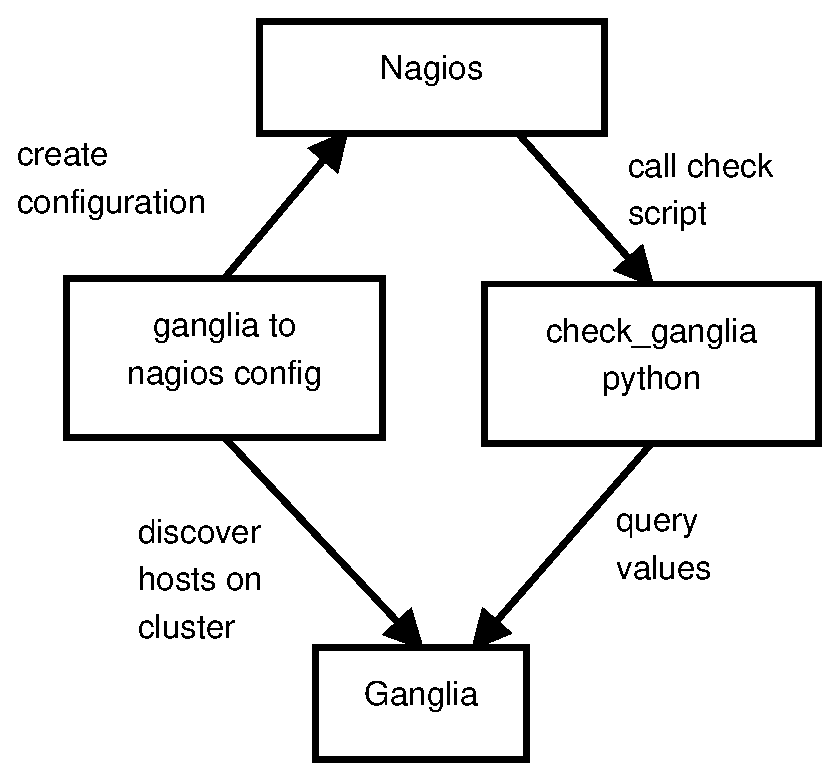
\includegraphics[width=80mm]{images/nagios_check_ganglia.eps}
\caption{Nagios configuration and check ganglia values}
\label{figure:nagios_ganglia}
\end{figure}

To integrate Ganglia with Nagios as shown in Figure \ref{figure:nagios_ganglia}, a custom script has been created. This script queries the Gmond source for the current state of nodes of the cluster. The returned result is being transformed to a Nagios configuration file to configure the host check of the cluster nodes. The Nagios service checks for these hosts are preconfigured. Script source may be found in Listing \ref{nagios_script}.

\begin{lstlisting}[language=bash,caption=Ganglia to Nagios script,label=nagios_script]
#!/bin/bash
if [ ! $1 ]
then
        echo "Please HOST argument"
        echo "ex. ganglia_to_nagios 10.0.0.1"
        exit
fi
/usr/src/redhat/SOURCES/ganglia-python-3.3.0/ganglia.py --host $1 --live | while read host
do
        echo ";$host.oslab.teipir.gr
define host{
        use     gmond-host
        host_name       $host.oslab.teipir.gr
        alias           $host
        address         $host.oslab.teipir.gr
        hostgroups      worker-nodes
}
"
done > /etc/nagios/teipir/hosts.cfg
\end{lstlisting}

When a nagios check command is executed, results are stored in a file, and Performance Data are calculated by a perl script. To scale this process, the Bulk Mode method is used to move the file to a spool directory which takes place immediately with no important performance impact to the system, because its only an inode operation. The NPCD (Nagios Performance C Daemon) is a daemon that is running on the Nagios host and its role is to monitor a spool directory for new files and pass the names of the files to process\_perfdata.pl. The script processes the performance data, and this operation is fully Nagios independent so it may be scaled-out more easily. Results are finally delivered to RRDTool, and graphs are being generated. This process is presented in Figure \ref{figure:pnp4nagios}

\begin{figure}[htb]
\centering
 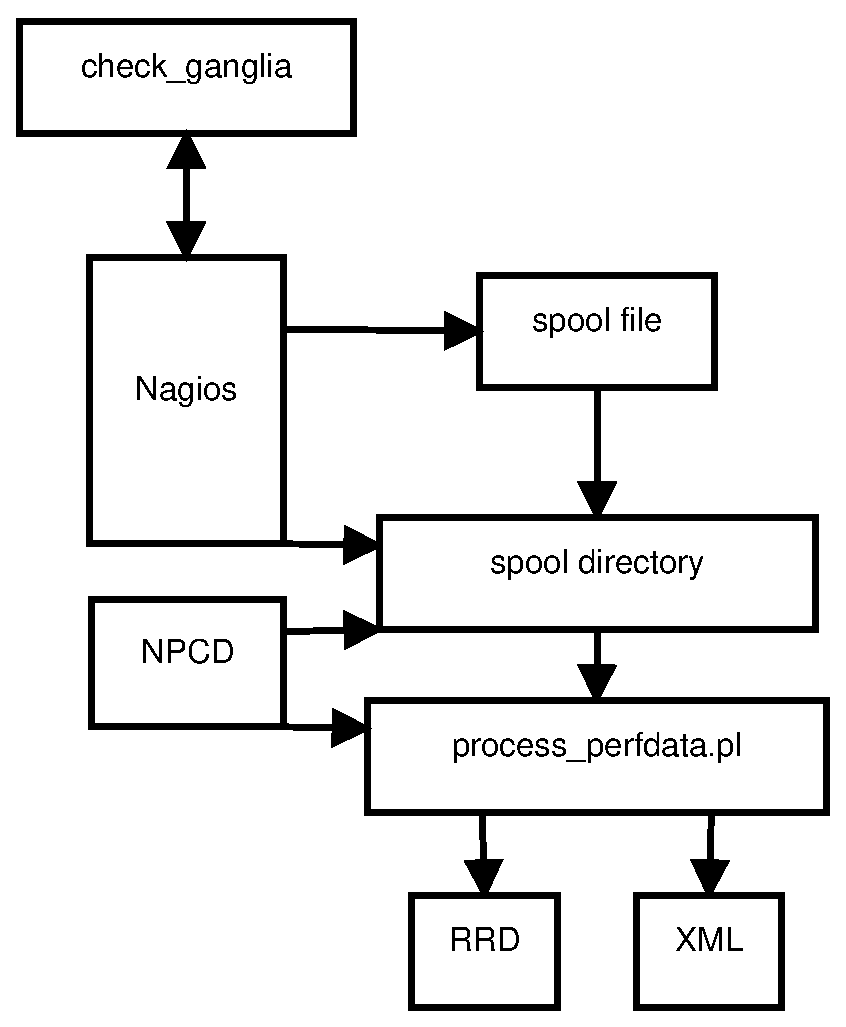
\includegraphics[width=80mm]{images/npcd_pnp4nagios.eps}
\caption{PNP 4 Nagios data flow}
\label{figure:pnp4nagios}
\end{figure}

\section{Range of cases examined}

To deliver Ganglia metrics, two different information systems were evaluated:
\begin{itemize}
  \item {\bf BDII}, which is used by gLite and is based on {\bf LDAP} and
  \item {\bf WSRF}, the framework that Globus uses to aggregate and deliver information using {\bf Web Services}.
\end{itemize}

Both Information Services are following the MDS specification and are using the Glue Schema to present the results of the metrics that are aggregated in its store.

\subsection{LDAP based}

To evaluate the LDAP based information service, a system should have the gLite installed and the BDII service running. To do this, a Scientific Linux installation were used, and CERN repositories were added. The installation of gLite-UI automatically installs BDII, and by using {\bf yum command} the needed packages were installed. An ldapsearch returned the top elements of the BDII as shown below:

\begin{lstlisting}
[root@osweb~]# ldapsearch -x -h osweb.teipir.gr -p 2170 -b "" -s base "(objectClass=*)" namingContexts
namingContexts: o=grid
namingContexts: o=glue
namingContexts: o=infosys
\end{lstlisting}

To test the connection to the Gmond service over TCP, and the transformation to MDS, two different ways were used:

\begin{enumerate}
\item The official ganglia python client, and
\item A perl script that is doing the same transformation
\end{enumerate}

\begin{lstlisting}
# /usr/bin/ganglia --host mon.oslab.teipir.gr --format=MDS
dn: mds-vo-name=local, o=grid
objectclass: GlueTop
objectclass: GlueGeneralTop
GlueSchemaVersionMajor: 1
GlueSchemaVersionMinor: 1
\end{lstlisting}

\begin{lstlisting}
# /root/ganglia_ip -h mon.oslab.teipir.gr -p 8649 -o mds
dn: GlueHostName=gr02.oslab.teipir.gr, mds-vo-name=local, o=grid
objectclass: GlueHost
GlueHostName: gr02.oslab.teipir.gr
GlueHostUniqueID: RDLAB-TEIPIR-gr02.oslab.teipir.gr
objectclass: GlueHostProcessorLoad
GlueHostProcessorLoadLast1Min: 1
GlueHostProcessorLoadLast5Min: 1
GlueHostProcessorLoadLast15Min: 0
\end{lstlisting}

As we can see, the LDIF exported by these tools, follows the schema defined by the Glue specification, whose attributes and objectclasses were extended by Glue-CE ProcessorLoad as shown in Table \ref{tab:glue}.

\begin{table}[ht]
\small\addtolength{\tabcolsep}{-3pt}
\scalebox{0.82}{
\begin{tabular}{ | l | l | l |}
\hline
{\bf Common Name} & {\bf Attribute} & {\bf Objectclass} \\ \hline
Hostname & GlueHostName & GlueHost \\ \hline
Unique ID assigned to the host & GlueHostUniqueID & GlueHost  \\ \hline
Processor Load, 1 Min Average  & GlueHostProcessorLoadLast1Min & GlueHostProcessorLoad \\ \hline
Processor Load, 5 Min Average  & GlueHostProcessorLoadLast5Min & GlueHostProcessorLoad \\ \hline
Processor Load, 15 Min Average  & GlueHostProcessorLoadLast15Min & GlueHostProcessorLoad \\ \hline
SMP Load, 1 Min Average  & GlueHostSMPLoadLast1Min & GlueHostSMPLoad \\ \hline
SMP Load, 5 Min Average  & GlueHostSMPLoadLast5Min & GlueHostSMPLoad \\ \hline
SMP Load, 15 Min Average  & GlueHostSMPLoadLast15Min & GlueHostSMPLoad \\ \hline
Number of CPUs  & GlueHostArchitectureSMPSize & GlueHostArchitecture \\ \hline
Processor Clock Speed (MHz)  & GlueHostProcessorClockSpeed & GlueHostProcessor \\ \hline
Network Interface name  & GlueHostNetworkAdapterName & GlueHostNetworkAdapter \\ \hline
Network Adapter IP address  & GlueHostNetworkAdapterIPAddress & GlueHostNetworkAdapter \\ \hline
The amount of RAM  & GlueHostMainMemoryRAMSize & GlueHostMainMemory \\ \hline
Free RAM (in KBytes)  & GlueHostMainMemoryRAMAvailable & GlueHostMainMemory \\ \hline
\end{tabular}}
\caption{GLUE schema for Host Processor Information Provider}
\label{tab:glue}
\end{table}

Finally, BDII was configured using {\bf yaim} with site-info definitions as shown below:

\begin{lstlisting}
# cat site-info.def
CE_HOST="osweb.teipir.gr"
SITE_BDII_HOST="osweb.teipir.gr"
SITE_EMAIL="theofpa@teipir.gr"
SITE_LAT=37.979166
SITE_LONG=23.674719
SITE_DESC="TEI of Piraeus"
SITE_LOC="Athens, Greece"
SITE_WEB="http://oslab.teipir.gr"
SITE_SECURITY_EMAIL=$SITE_EMAIL
SITE_SUPPORT_EMAIL=$SITE_EMAIL
SITE_OTHER_GRID="EGEE"
BDII_REGIONS="oslab.teipir.gr"
# /opt/glite/yaim/bin/yaim -c -s site-info.def -n BDII_site
\end{lstlisting}

In order to integrate Ganglia with MDS in early versions of Globus and BDII of gLite, the schema of OpenLDAP should be extended using the Glue-CE definitions from the DataTAG web site (MDS version 2.4). The Ganglia Information Provider that was used is a ganglia client on perl, and not the python client given by the ganglia development team it shelf.

gLite has a dedicated directory for information providers, where the wrappers of each provider reside. An one-line wrapper to call the perl script was created, to use the information provider with BDII as shown below:

\begin{lstlisting}
[root@osweb ~]# ps -ef |grep bdi[i]
edguser  24951     1  0 Feb16 ?        00:00:23 /usr/sbin/slapd -f /opt/bdii/etc/bdii-slapd.conf -h ldap://osweb.teipir.gr:2170 -u edguser
edguser  24990     1  0 Feb16 ?        00:01:00 /usr/bin/python /opt/bdii/bin/bdii-update -c /opt/bdii/etc/bdii.conf -d
[root@osweb ~]# grep PROVIDER /opt/bdii/etc/bdii.conf
BDII_PROVIDER_DIR=/opt/glite/etc/gip/provider
[root@osweb ~]# cat /opt/glite/etc/gip/provider/glite-provider-ganglia-wrapper
#!/bin/bash
/opt/bin/ganglia_ip -h 195.251.70.54 -p 8649 -o mds
\end{lstlisting}

\subsection{Web Service based - WSRF}

Globus on the other hand, since version 4 and later provides the Web Service Resource Framework that offers a scalable information system with build-in aggregation framework and index service as shown in Figure \ref{figure:wsrf}. WSRF is an OASIS organization standard and follows the Glue schema and MDS specification.

\begin{figure}[htb]
\centering
 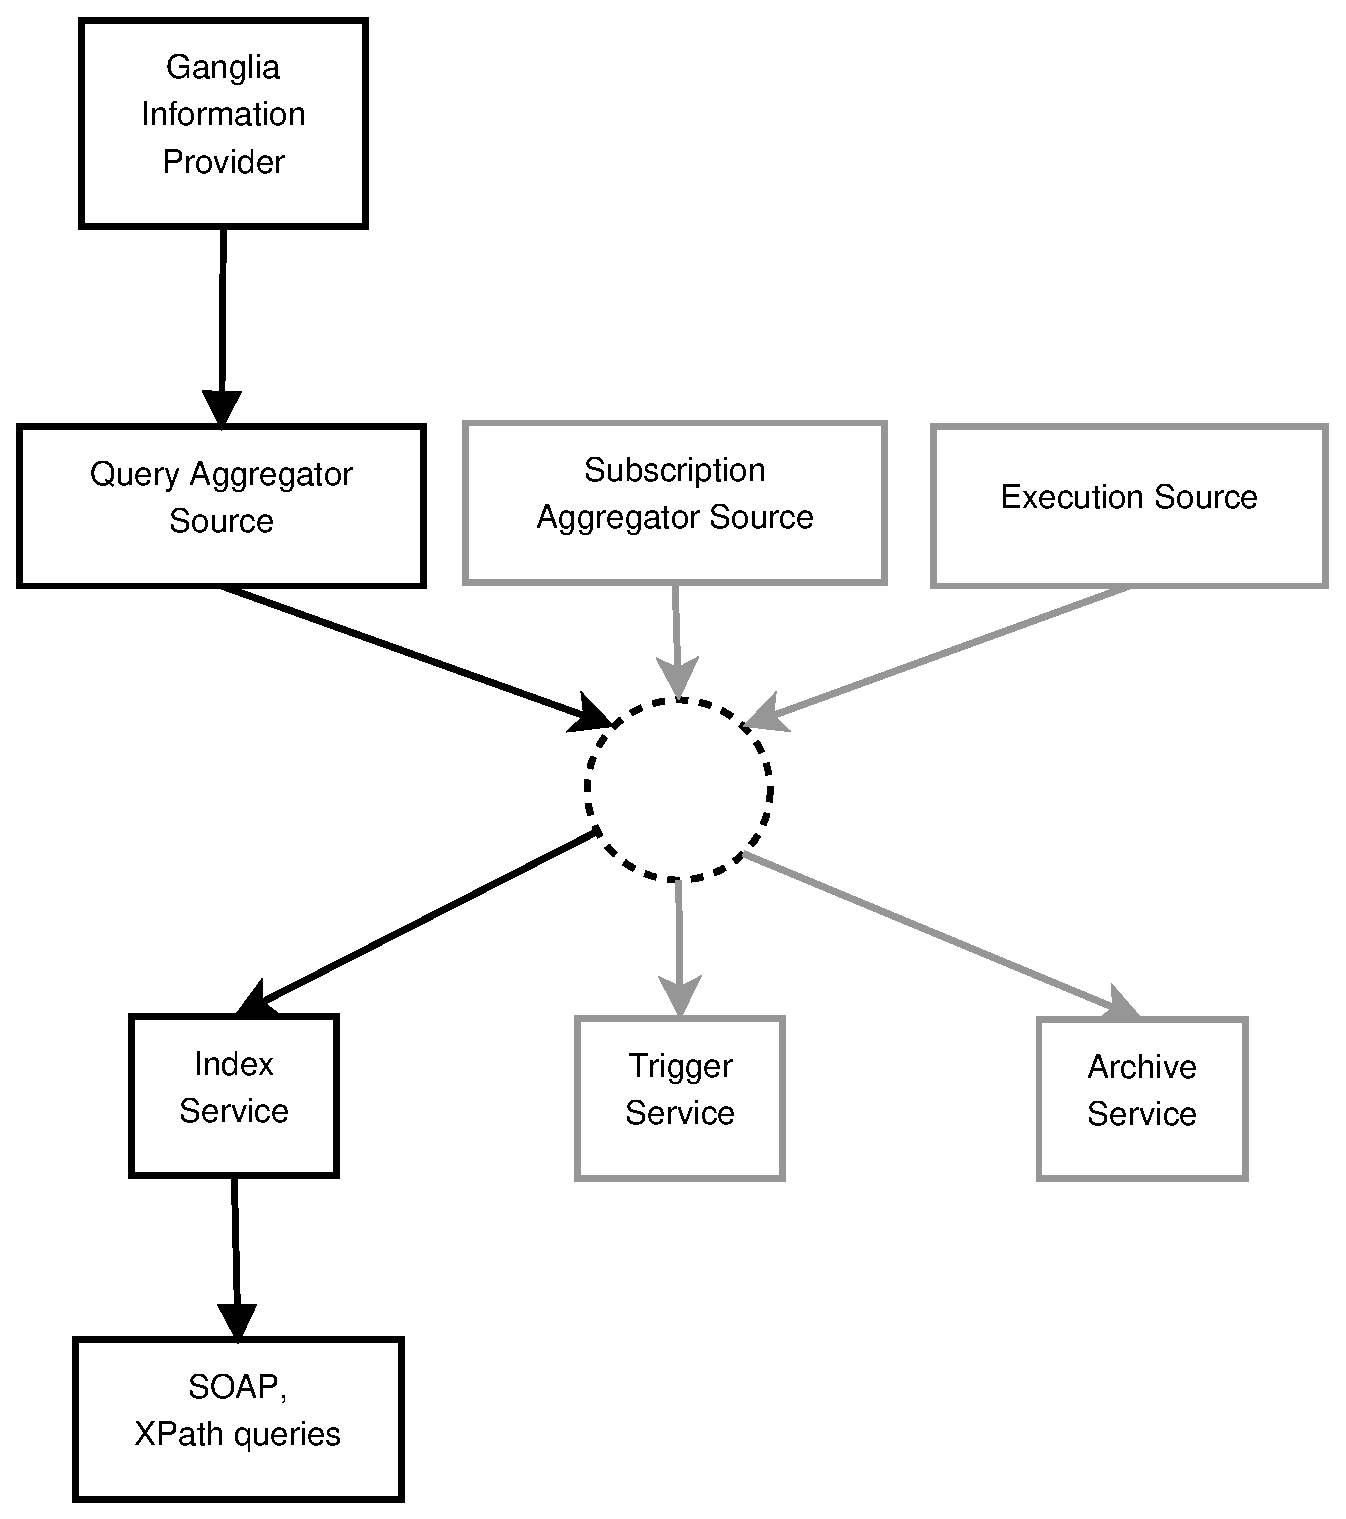
\includegraphics[width=120mm]{images/wsrf.eps}
\caption{Web Service Resource Framework}
\label{figure:wsrf}
\end{figure}

Globus Toolkit version 4.0.7 was used to install WSRF, by extracting its binary distribution in the target system. A PostgreSQL database was installed and a special user and DB was created to host the RFT schema and data in order to have a minimal globus environment and start the container to service WSRF. A custom start/stop script was created for that container and the file rpprovider-config-gluece.xml was created as shown in Listing \ref{wsrfrp}.

\begin{lstlisting}[language=XML,caption=Ganglia Resource Provider for WSRF Index,label=wsrfrp]
<ns1:ResourcePropertyProviderConfigArray xsi:type="ns1:ResourcePropertyProviderConfigArray" xmlns:ns1="http://mds.globus.org/rpprovider/2005/08" xmlns:xsi="http://www.w3.org/2001/XMLSchema-instance">
 <ns1:configArray xsi:type="ns1:resourcePropertyProviderConfig">
  <ns1:resourcePropertyName xsi:type="xsd:QName" xmlns:mds="http://mds.globus.org/glue/ce/1.1">mds:GLUECE</ns1:resourcePropertyName>
  <ns1:resourcePropertyImpl xsi:type="xsd:string">org.globus.mds.usefulrp.rpprovider.GLUEResourceProperty</ns1:resourcePropertyImpl>
  <ns1:resourcePropertyElementProducers xsi:type="ns1:resourcePropertyElementProducerConfig">
    <ns1:className xsi:type="xsd:string">org.globus.mds.usefulrp.glue.GangliaElementProducer</ns1:className>
    <ns1:arguments xsi:type="xsd:string">195.251.70.55</ns1:arguments>
    <ns1:arguments xsi:type="xsd:string">8649</ns1:arguments>
    <ns1:period xsi:type="xsd:int">60</ns1:period>
    <ns1:transformClass xsi:type="xsd:string">org.globus.mds.usefulrp.rpprovider.transforms.GLUEComputeElementTransform</ns1:transformClass>
  </ns1:resourcePropertyElementProducers>
  <ns1:resourcePropertyElementProducers xsi:type="ns1:resourcePropertyElementProducerConfig">
    <ns1:className xsi:type="xsd:string">org.globus.mds.usefulrp.rpprovider.producers.SchedulerInfoElementProducer</ns1:className>
    <ns1:arguments xsi:type="xsd:string">libexec/globus-scheduler-provider-fork</ns1:arguments>
    <ns1:transformClass xsi:type="xsd:string">org.globus.mds.usefulrp.rpprovider.transforms.GLUESchedulerElementTransform</ns1:transformClass>
    <ns1:period xsi:type="xsd:int">300</ns1:period>
  </ns1:resourcePropertyElementProducers>
 </ns1:configArray>
</ns1:ResourcePropertyProviderConfigArray>
\end{lstlisting}

File rpprovider-config-gluece.xml was included by the server-config.wsdd of the container as shown in Listing \ref{wsrfwsdd}.

\begin{lstlisting}[language=XML,caption=Web Service Deployment Descriptor for WSRF Index,label=wsrfwsdd]
<service name="DefaultIndexService" provider="Handler" use="literal" style="document">
 <parameter name="providers"
  value="org.globus.mds.usefulrp.rpprovider.ResourcePropertyProviderCollection
  org.globus.wsrf.impl.servicegroup.ServiceGroupRegistrationProvider
  GetRPProvider
  GetMRPProvider
  QueryRPProvider
  DestroyProvider
  SetTerminationTimeProvider
  SubscribeProvider
  GetCurrentMessageProvider"/>
 <parameter name="rpProviderConfigFile" value="/etc/globus_wsrf_mds_index/rpprovider-config-gluece.xml"/>
 <parameter name="handlerClass" value="org.globus.axis.providers.RPCProvider"/>
 <parameter name="scope" value="Application"/>
 <parameter name="allowedMethods" value="*"/>
 <parameter name="className"
  value="org.globus.mds.index.impl.DefaultIndexService"/>
 <wsdlFile>share/schema/mds/index/index_service.wsdl</wsdlFile>
</service>
\end{lstlisting}

When the container started, a user proxy certificate was initialised and an XPath query was issued to test the integration:
 
\begin{lstlisting}[caption=WSRF command line query]
[root@osweb ~]# /opt/globus/bin/grid-proxy-init
Your identity: /C=GR/O=HellasGrid/OU=teipir.gr/CN=Theofylaktos Papapanagiotou
Enter GRID pass phrase for this identity:
Creating proxy ................................... Done
Your proxy is valid until: Thu Feb 17 11:11:59 2011
[root@osweb ~]# /opt/globus/bin/wsrf-query -s https://osweb.teipir.gr:8443/wsrf/services/DefaultIndexService "//*[local-name()='Host']"
<ns1:Host ns1:Name="gr02.oslab.teipir.gr" ns1:UniqueID="gr02.oslab.teipir.gr" xmlns:ns1="http://mds.globus.org/glue/ce/1.1">
 <ns1:Processor ns1:CacheL1="0" ns1:CacheL1D="0" ns1:CacheL1I="0" ns1:CacheL2="0" ns1:ClockSpeed="2527" ns1:InstructionSet="x86"/>
 <ns1:MainMemory ns1:RAMAvailable="75" ns1:RAMSize="495" ns1:VirtualAvailable="1129" ns1:VirtualSize="1559"/>
 <ns1:OperatingSystem ns1:Name="Linux" ns1:Release="2.6.18-194.26.1.el5"/>
 <ns1:Architecture ns1:SMPSize="1"/>
 <ns1:FileSystem ns1:AvailableSpace="34082" ns1:Name="entire-system" ns1:ReadOnly="false" ns1:Root="/" ns1:Size="38624"/>
 <ns1:NetworkAdapter ns1:IPAddress="10.0.0.32" ns1:InboundIP="true" ns1:MTU="0" ns1:Name="gr02.oslab.teipir.gr" ns1:OutboundIP="true"/>
 <ns1:ProcessorLoad ns1:Last15Min="0" ns1:Last1Min="0" ns1:Last5Min="0"/>
\end{lstlisting}

\subsubsection{XPath}

XPath is used to parse an XML document and get a part of it using an address scheme. XPath considers XML document as a tree, consisting of nodes. Its purpose as a language is to get from that document, the nodes that are addressed using the XPath query.

Its syntax is compact, non-XML and much like the filesystem addressing, so it facilitates the use of XPath within URIs.

Example queries used in this project are:

The following is used in the PHP code that queries the WebMDS for all nodes of the XML of the WSRF containing nodes with name $Host$:
\begin{lstlisting}
//*[local-name()='Host']
\end{lstlisting}

Another example is a more complex query that asks the WSRF for all nodes by the name $Host$ that contains a sub-node named $ProcessorLoad$ and its $Last15Min$ attribute has value larger than 20:
\begin{lstlisting}
//glue:Host[glue:ProcessorLoad[@glue:Last15Min>20]]
\end{lstlisting}

Finally the following example may return only the $ProcessorLoad$ node of the $Host$ that has the attribute Name set to $xenia.oslab.teipir.gr$:
\begin{lstlisting}
//glue:Host[@glue:Name='xenia.oslab.teipir.gr']/glue:ProcessorLoad
\end{lstlisting}


\subsubsection{WebMDS}

WebMDS is a web interface to query WSRF resource property information. It consists of forms and views of raw XML or organized in tables of results. This user friendly frontend comes as a part of Globus Toolkit version 4 and it can be deployed in any application server. Behind this application reside the data that the WSRF aggregation framework provides through the Index Service.

\begin{figure}[htb]
\centering
 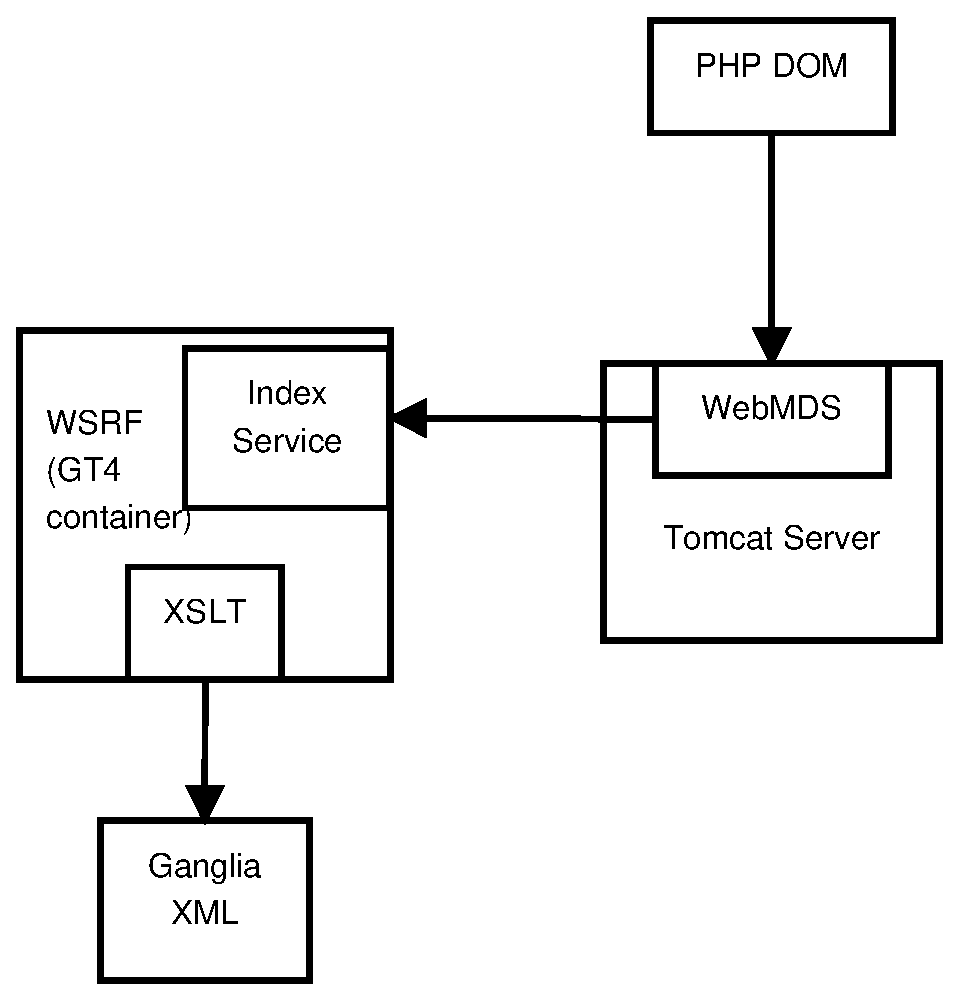
\includegraphics[width=80mm]{images/webmds.eps}
\caption{WebMDS application}
\label{figure:webmds}
\end{figure}

Figure \ref{figure:webmds} display the data flow of the WSRF Information System case. The PHP from Brunel's web server calls WebMDS and get the result in XML which parses using DOM. WebMDS is deployed in the Tomcat container, and calls the Index Service of WSRF which is deployed in the GT4 container. WSRF connects (if cache has expired) to the Gmond process and transforms the data received using XSLT.

For this project an Apache Tomcat server was installed in the box that globus toolkit was running, and the {\bf webmds application} from the GT4 home was deployed. In webmds configuration file, the global option to allow user specified queries using XPath was enabled.

\begin{lstlisting}
[root@osweb ~]# cat /opt/globus/lib/webmds/globalconfig.xml 
<WebmdsGlobalConfig>
  <newStyleErrors>true</newStyleErrors>
  <allowUserSpecifiedQuery>true</allowUserSpecifiedQuery>
</WebmdsGlobalConfig>
\end{lstlisting}
